\documentclass[@BEAMER_OPTIONS@]{beamer}
    @USE_PGFPAGES@

    \usetheme[alternativetitlepage=true,titleline=true]{Torino}
    \setbeamertemplate{navigation symbols}{}
    \setbeamertemplate{note page}[plain]

    \usepackage[utf8]{inputenc}
    \usepackage[russian]{babel}
    \usepackage{graphicx}
    \usepackage{subfigure}
    \usepackage{xspace}
    \usepackage{adjustbox}
    \usepackage{tikz}
    \usepgflibrary{arrows}
    \usetikzlibrary{shadows,decorations.pathreplacing,patterns,shapes}
    \tikzstyle{every picture}=[semithick,>=stealth,remember picture]
    \usepackage{listings}
    \lstset{
        language=C++,
        basicstyle=\footnotesize\rmfamily,
        stringstyle=\color{chameleon4},
        numbers=left,
        numberstyle=\tiny,
        aboveskip=-0.02\baselineskip,
        belowskip=-0.02\baselineskip,
        columns=flexible,
        extendedchars=false,
        showstringspaces=false
        }
    \newcommand{\code}[1]{\lstinline|#1|}
    \newcommand{\additive}{\hspace{1cm}\footnotesize(\emph{Additive expressions only})}
    \newcommand{\Cpp}{{C\nolinebreak[4]\hspace{-.05em}\raisebox{.4ex}{\tiny\bf ++}}\xspace}
    \newcommand{\ghribbon}{
        \begin{tikzpicture}[remember picture,overlay]
            \node[anchor=north east,yshift=4pt,xshift=4pt] at (current page.north east) {
                \href{https://github.com/ddemidov/vexcl}{
\includegraphics[width=2cm]{forkme}}
            };
        \end{tikzpicture}
    }

    \title{Автоматическая генерация вычислительных ядер OpenCL\newline
с помощью библиотеки VexCL}

    \author{Денис Демидов}
    \institute{
        Казанский Федеральный Университет,\\
        Межведомственный суперкомпьютерный центр РАН
    }
    \date{Абрау-Дюрсо 2013}


\begin{document}

%----------------------------------------------------------------------------
\begin{frame}{}
    \titlepage
\end{frame}

\note{ }

%----------------------------------------------------------------------------
\begin{frame}{Современные GPGPU платформы}
    \begin{columns}
        \begin{column}{0.45\textwidth}
            \begin{block}{NVIDIA CUDA}
                \begin{itemize}
                    \item Проприетарная архитектура
                    \item Необходимо аппаратное обеспечение NVIDIA
                    \item Зрелое окружение, большое число библиотек
                        \vspace{\baselineskip}
                    \item<2> \emph{Ядра компилируются в псевдо-ассемблер (PTX)
                        вместе с основной программой}
                \end{itemize}
            \end{block}
        \end{column}
        \begin{column}{0.45\textwidth}
            \begin{block}{OpenCL}
                \begin{itemize}
                    \item Открытый стандарт
                    \item Большой диапазон поддерживаемого железа
                    \item Низкоуровневый программный интерфейс
                        \vspace{\baselineskip}
                    \item<2> \emph{Ядра компилируются во время выполнения,
                            увеличивается время инициализации}
                \end{itemize}
            \end{block}
        \end{column}
    \end{columns}
    \vspace{\baselineskip}
    \begin{itemize}
        \item<2> Последнее отличие обычно считается недостатком OpenCL.
        \item<2> Однако, это позволяет генерировать во время выполнения более
            эффективные ядра под конкретную задачу!
    \end{itemize}
\end{frame}

\note{ }

%----------------------------------------------------------------------------
\begin{frame}{}
    \tableofcontents
\end{frame}

\note{ }

\section{Обзор интерфейса VexCL}

%----------------------------------------------------------------------------
\begin{frame}{VexCL: библиотека шаблонов векторных выражений для OpenCL}
    \ghribbon
    \begin{itemize}
        \item \href{https://github.com/ddemidov/vexcl}{https://github.com/ddemidov/vexcl}
            \vspace{\baselineskip}
        \item Создана для облегчения разработки OpenCL приложений на \Cpp.
            \begin{itemize}
                \item Интуитивная нотация для записи векторных выражений.
                \item Автоматическая генерация кода OpenCL.
            \end{itemize}
        \item Исходный код доступен под лицензией MIT.
    \end{itemize}
\end{frame}

\note[itemize]{
\item VexCL is a vector expression template library for OpenCL. It uses
    template metaprogramming techniques (in particular, expression templates)
    to provide an intuitive notation for vector and matrix operations.
\item The source code of the library is available on GitHub. It is distributed
    under MIT license, so you are basically free to do whatever you want with
    the library.
\item I would like to note that this is not another \Cpp bindings library. VexCL
    is designed to work with standard \Cpp bindings for OpenCL that are provided
    by the Khronos group.
}

%----------------------------------------------------------------------------
\begin{frame}[fragile]{Hello VexCL: сумма векторов}
    \setbeamercovered{transparent=40}
    \begin{exampleblock}{Инициализация контекста:}
        \begin{lstlisting}
vex::Context ctx( vex::Filter::Type(CL_DEVICE_TYPE_GPU) );
if ( !ctx ) throw std::runtime_error("GPUs not found");
        \end{lstlisting}
    \end{exampleblock}
    \pause
    \begin{exampleblock}{Подготовка входных данных, перенос на GPU:}
        \begin{lstlisting}[firstnumber=last]
std::vector<float> a(N, 1), b(N, 2), c(N);
vex::vector<float> A(ctx, a);
vex::vector<float> B(ctx, b);
vex::vector<float> C(ctx, N);
        \end{lstlisting}
    \end{exampleblock}
    \pause
    \begin{exampleblock}{Запуск вычислительного ядра, перенос результатов на
        CPU:}
        \begin{lstlisting}[firstnumber=last]
C = A + B;
vex::copy(C, c);
std::cout << c[42] << std::endl;
        \end{lstlisting}
    \end{exampleblock}
\end{frame}

\note[itemize]{
\item Here is the simplest example of using vexcl: addition of two vectors on a
    gpu card.
\item First, we initialize VexCL context. We provide a device filter to the
    context constructor and get all compute devices that satisfy the filter.
    Here we filter by type and get all available GPUs.
\item Next, we allocate device vectors and transfer input data to devices.
\item Finally, we sum the input vectors in line 7. This simple expression leads
    to automatic generation and launch of OpenCL kernel.  Then we copy the
    results back to host and see what we got.
}

%----------------------------------------------------------------------------
\begin{frame}[fragile]{Разделение памяти и работы между устройствами}
    \setbeamercovered{transparent=40}
    \begin{exampleblock}{}
        \begin{onlyenv}<1|handout:0>
        \begin{lstlisting}[escapechar=!]
vex::Context ctx( vex::Filter::Name("Tesla") );
        \end{lstlisting}
        \end{onlyenv}
        \begin{onlyenv}<2|handout:0>
        \begin{lstlisting}[escapechar=!]
vex::Context ctx( vex::Filter::Type(CL_DEVICE_TYPE_GPU) );
        \end{lstlisting}
        \end{onlyenv}
        \begin{onlyenv}<3>
        \begin{lstlisting}[escapechar=!]
vex::Context ctx( vex::Filter::DoublePrecision );
        \end{lstlisting}
        \end{onlyenv}
        \begin{uncoverenv}<1>
        \begin{lstlisting}[firstnumber=last]

vex::vector<float> A(ctx, N); A = 1;
vex::vector<float> B(ctx, N); B = 2;
vex::vector<float> C(ctx, N);

C = A + B;
        \end{lstlisting}
        \end{uncoverenv}
    \end{exampleblock}
    \setbeamercovered{invisible}
    \begin{figure}
        \begin{tikzpicture}
            \draw (0,3.0) rectangle +(8,0.1);
            \draw (0,3.0) grid[step=0.1] +(8,0.1);
            \draw (-0.3,3.1) node{A};

            \draw (0,2.5) rectangle +(8,0.1);
            \draw (0,2.5) grid[step=0.1] +(8,0.1);
            \draw (-0.3,2.6) node{B};

            \draw (0,2.0) rectangle +(8,0.1);
            \draw (0,2.0) grid[step=0.1] +(8,0.1);
            \draw (-0.3,2.1) node[anchor=center]{C};

            \uncover<1-3> {
            \draw (1,0.5) node{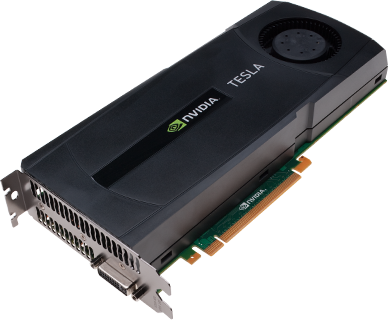
\includegraphics[width=0.2\textwidth]{tesla.png}};
            }

            \uncover<2-3> {
            \draw (4,0.5) node{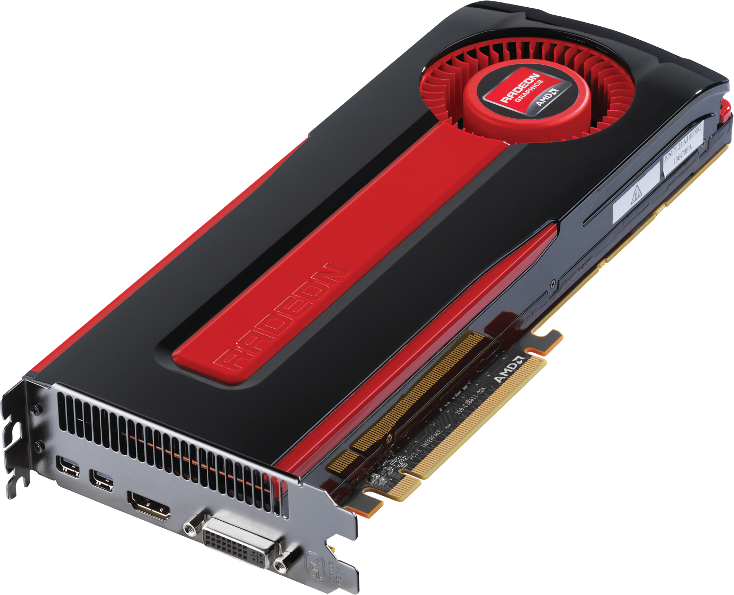
\includegraphics[width=0.2\textwidth]{radeon.png}};
            }

            \uncover<3> {
            \draw (7.5,0.5) node{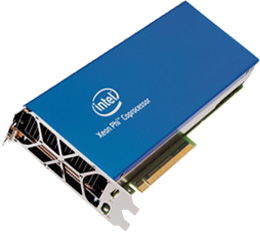
\includegraphics[width=0.16\textwidth]{intel.png}};
            }

            \uncover<1|handout:0> {
            \draw[->,chameleon3,style=dashed] (0,3.2) -- (0,1.8)
                .. controls +(east:0.5) and +(north west:0.5) ..
                (1.4,1.5);
            \draw[->,chameleon3,style=dashed] (8,3.2) -- (8,1.8)
                .. controls +(west:0.5) and +(north east:0.5) ..
                (1.6,1.5);
            }

            \uncover<2|handout:0> {
            \draw[->,chameleon3,style=dashed] (0,3.2) -- (0,1.8)
                .. controls +(east:0.5) and +(north west:0.5) ..
                (1.4,1.5);
            \draw[->,chameleon3,style=dashed] (4,3.2) -- (4,1.8)
                .. controls +(west:0.5) and +(north east:0.5) ..
                (1.6,1.5);

            \draw[->,chameleon3,style=dashed] (4,3.2) -- (4,1.8)
                .. controls +(east:0.1) and +(north west:0.2) ..
                (4.4,1.5);
            \draw[->,chameleon3,style=dashed] (8,3.2) -- (8,1.8)
                .. controls +(west:0.5) and +(north east:0.5) ..
                (4.6,1.5);
            }

            \uncover<3> {
            \draw[->,chameleon3,style=dashed] (0,3.2) -- (0,1.8)
                .. controls +(east:0.5) and +(north west:0.5) ..
                (1.4,1.5);
            \draw[->,chameleon3,style=dashed] (3.5,3.2) -- (3.5,1.8)
                .. controls +(west:0.5) and +(north east:0.5) ..
                (1.6,1.5);

            \draw[->,chameleon3,style=dashed] (3.5,3.2) -- (3.5,1.8)
                .. controls +(east:0.5) and +(north west:0.2) ..
                (4.4,1.5);
            \draw[->,chameleon3,style=dashed] (7,3.2) -- (7,1.8)
                .. controls +(west:0.5) and +(north east:0.5) ..
                (4.6,1.5);

            \draw[->,chameleon3,style=dashed] (7,3.2) -- (7,1.8) -- (7.4,1.5);
            \draw[->,chameleon3,style=dashed] (8,3.2) -- (8,1.8) -- (7.6,1.5);
            }
        \end{tikzpicture}
    \end{figure}
\end{frame}

\note[itemize]{
\item The memory and the workload is split between all devices in VexCL
    context. The share that each device gets is by default proportional to the
    device's bandwidth.
    \begin{enumerate}
        \item For example, if we only have the Tesla card in our context, then
            it will hold the complete memory for all of our vectors.
        \item If we use both of the available GPUs, then the vectors will be
            split between the devices. This split is by default proportional to
            the GPU bandwidth and is guaranteed to be consistent for vectors of
            the same size. This consistency allows VexCL to run computations
            independently on all devices in context.
        \item If we add the CPU to the context, it will get smaller share of
            the data and arithmetic operations.
    \end{enumerate}
}

%----------------------------------------------------------------------------
\begin{frame}[fragile]{Допустимые векторные выражения}
    \begin{itemize}
        \item Все векторы в выражении должны быть \emph{совместимыми}:
            \begin{itemize}
                \item Иметь один размер
                \item Быть расположенными на одних и тех же устройствах
            \end{itemize}
        \item Что можно использовать в выражениях:
            \begin{columns}
                \begin{column}{0.4\textwidth}
                    \begin{itemize}
                        \item Векторы и скаляры
                        \item Арифм. и логич. операторы
                        \item Встроенные функции OpenCL
                        \item Пользовательские функции
                        \item Генераторы случайных чисел
                    \end{itemize}
                \end{column}
                \begin{column}{0.4\textwidth}
                    \begin{itemize}
                        \item Временные значения
                        \item Срезы и перестановки
                        \item Редукция (сумма, экстремумы)
                        \item Произв. матрицы на вектор
                        \item Быстрое преобразование Фурье
                    \end{itemize}
                \end{column}
            \end{columns}
    \end{itemize}
    \begin{exampleblock}{}
        \begin{lstlisting}
vex::vector<double> x(ctx, n), y(ctx, n);

x = (2 * M_PI / n) * vex::element_index();
y = pow(sin(x), 2.0) + pow(cos(x), 2.0);
        \end{lstlisting}
    \end{exampleblock}
\end{frame}

\note[itemize]{
\item So, what kind of expressions can you use in VexCL?
\item First, any vectors used in an expression have to be compatible.
\item If this requirement is satisfied, then expressions may combine
    vectors and scalars with almost any binary operators. OpenCL math functions
    and user-defined functions are also available.
}

%----------------------------------------------------------------------------
\begin{frame}[fragile]{Автоматическая генерация кода OpenCL}
    \begin{columns}
        \begin{column}{0.38\textwidth}
            \begin{exampleblock}{Выражение}
                \begin{lstlisting}
x = 2 * y - sin(z);
                \end{lstlisting}
            \end{exampleblock}
        \end{column}
        \begin{column}{0.55\textwidth}
            \begin{itemize}
                \item \code{\#define VEXCL_SHOW_KERNELS}\\ для вывода
                    сгенерированного кода.
            \end{itemize}
        \end{column}
    \end{columns}
    \begin{exampleblock}{\ldots приводит к генерации и выполнению ядра:}
        \begin{lstlisting}
kernel void vexcl_vector_kernel(
    ulong n,
    global double * res,
    int prm1,
    global double * prm2,
    global double * prm3
)
{
    for(size_t idx = get_global_id(0); idx < n; idx += get_global_size(0)) {
        res[idx] = ( ( prm1 * prm2[idx] ) - sin( prm3[idx] ) );
    }
}
        \end{lstlisting}
    \end{exampleblock}
    \begin{tikzpicture}[overlay,scale=0.6]
        \draw (16,8) node(sub)[draw,fill=white,ellipse,drop shadow]{$-$};

        \draw (sub) +(-2.00,-1.5) node(mul)[draw,fill=white,drop shadow,ellipse]{$*$};
        \draw (sub) +( 2.00,-1.5) node(sin)[draw,fill=white,drop shadow,ellipse]{sin};
        \draw (mul) +(-2.00,-1.5) node(two)[draw,fill=white,drop shadow,minimum size=0.5cm]{2};
        \draw (mul) +( 2.00,-1.5) node(y)  [draw,fill=white,drop shadow,minimum size=0.5cm]{y};
        \draw (sin) +( 0.00,-1.5) node(z)  [draw,fill=white,drop shadow,minimum size=0.5cm]{z};

        \draw (sub) -- (mul);
        \draw (sub) -- (sin);
        \draw (mul) -- (two);
        \draw (mul) -- (y);
        \draw (sin) -- (z);
    \end{tikzpicture}
\end{frame}

\note[itemize]{
\item Boost.Proto is used as an expression template engine.
\item Expression tree terminals become kernel parameters, and the expression
    string is formed from the information encoded in the expression tree.
\item If you are curious, you can define \code{VEXCL_SHOW_KERNELS} macro before
    vexcl include pragma. This will show sources for every generated kernel on
    standard output.
}

%----------------------------------------------------------------------------
\section{Модельная задача}

\begin{frame}{}
    \tableofcontents[currentsection]
\end{frame}

\note{
}

%----------------------------------------------------------------------------
\begin{frame}[fragile]{Параметрическое исследование системы Лоренца}
    \begin{columns}
        \begin{column}{0.6\textwidth}
            \begin{block}{Система Лоренца}
                \vspace{-1\baselineskip}
                \begin{align*}
                    \dot{x} &= -\sigma \left( x - y \right), \\
                    \dot{y} &= R x - y - xz, \\
                    \dot{z} &= -bz + xy.
                    \label{eq:lorenz}
                \end{align*}
            \end{block}
            \begin{itemize}
                \item Будем одновременно решать большое число систем Лоренца
                    для различных значений $R$.
                \item Будем использовать библиотеки VexCL и Boost.odeint.
            \end{itemize}
        \end{column}
        \begin{column}{0.4\textwidth}
            \begin{figure}
                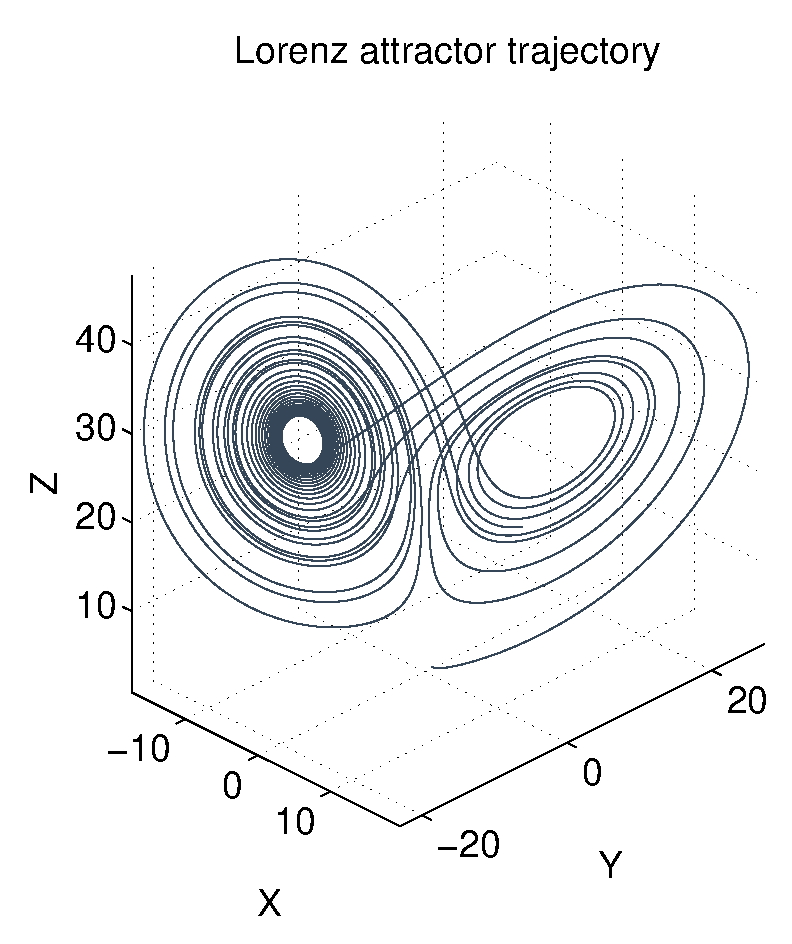
\includegraphics[width=\textwidth]{lorenz}
            \end{figure}
        \end{column}
    \end{columns}
\end{frame}

\note[itemize]{
\item As an example, lets solve a Lorenz attractor system of ordinary
    differential equations.
\item Lorenz attractor is a particle that moves according to these governing
    equations. The plot on the right shows an example of particle trajectory in
    time.
\item We will solve large number of these Lorenz systems at once.  Each of the
    systems will have its own value for parameter R. That's why this is called
    a parameter study.
}

%----------------------------------------------------------------------------
\begin{frame}{Использование Boost.odeint}
    \begin{block}{Общий вид ОДУ:}
        \begin{equation*}
            \frac{\mbox{d} x}{\mbox{d} t } = \dot{x} = f(x , t),
            \quad \quad x(0) = x_0.
        \end{equation*}
    \end{block}

    \vspace{\baselineskip}

    \begin{description}[\;]
        \item[Порядок применения Boost.odeint:] \quad
        \begin{enumerate}
            \item Определить тип переменной состояния (что такое $x$?)
            \item Определить системную функцию ($f$)
            \item Выбрать алгоритм интегрирования
            \item Выполнить интегрирование по времени
        \end{enumerate}
    \end{description}
\end{frame}

\note[itemize]{
\item Here is a general form of an ODE.
\item In order to use Boost.odeint, one has to...
}

\section{Простейшая реализация}

%----------------------------------------------------------------------------
\begin{frame}[fragile]{Простейшая реализация с VexCL}
    \begin{exampleblock}{1. Тип переменной состояния}
        \begin{lstlisting}
typedef vex::multivector<double, 3> state_type;
        \end{lstlisting}
    \end{exampleblock}

    \begin{exampleblock}{2. Системная функция}
        \begin{lstlisting}[firstnumber=last]
struct lorenz_system {
    const vex::vector<double> &R;
    lorenz_system(const vex::vector<double> &R ) : R(R) { }

    void operator()(const state_type &x, state_type &dxdt, double t) {
        dxdt = std::tie( sigma * ( x(1) - x(0) ),
                         R * x(0) - x(1) - x(0) * x(2),
                         x(0) * x(1) - b * x(2)  );
    }
};
        \end{lstlisting}
    \end{exampleblock}
\end{frame}

\note[itemize]{
\item We will hold current state of the system (or set of attractor
    coordinates) in a multivector with 3 components.
\item Here is the definition of the lorenz system functor: It computes the time
    derivative from current state and time (which is not used here).
\item VexCL make the definition of the functor very simple and intuitive: we
    assign a tuple of vector expressions to the multivector that represents
    time derivative.
}

%----------------------------------------------------------------------------
\begin{frame}[fragile]{Простейшая реализация с VexCL}
    \begin{exampleblock}{3. Алгоритм (Рунге-Кутты 4го порядка)}
        \begin{lstlisting}[firstnumber=last]
odeint::runge_kutta4<
        state_type /*state*/,      double /*value*/,
        state_type /*derivative*/, double /*time*/,
        odeint::vector_space_algebra, odeint::default_operations
        > stepper;
        \end{lstlisting}
    \end{exampleblock}
    \begin{exampleblock}{4. Интегрирование}
        \begin{lstlisting}[firstnumber=last]
vex::multivector<double, 3> X(ctx, n);
vex::vector<double> R(ctx, n);

X = 10;
R = Rmin + vex::element_index() * ((Rmax - Rmin) / (n - 1));

odeint::integrate_const(stepper, lorenz_system(R), X, 0.0, t_max, dt);
        \end{lstlisting}
    \end{exampleblock}
\end{frame}

\note[itemize]{
\item Next, we create the stepper object and run the integration routine. Here
    we use classic 4th order Runge-Kutta method.
\item And that's it! This was really easy.
\item And, as you will see from the next slide, it was an order of magnitude
    faster than a multithreaded CPU variant.
}

%----------------------------------------------------------------------------
\begin{frame}[fragile]{Вариант с использованием CUBLAS}
    \begin{itemize}
        \item CUBLAS~--- оптимизированная библиотека линейной алгебры от NVIDIA.
        \item Линейные комбинации (используемые в алгоритмах odeint):
            \begin{equation*}
                x_0 = \alpha_1 x_1 + \alpha_2 x_2 + \cdots + \alpha_n x_n
            \end{equation*}
            реализованы следующим образом:
    \end{itemize}
    \begin{exampleblock}{}
        \begin{lstlisting}[numbers=none]
cublasDcopy(...);
cublasDscal(...);
cublasDaxpy(...);
...
cublasDaxpy(...);
        \end{lstlisting}
    \end{exampleblock}
\end{frame}

%----------------------------------------------------------------------------
\begin{frame}[fragile]{Вариант с использованием Thrust}
    \begin{itemize}
        \item Thrust позволяет получить монолитное ядро:
    \end{itemize}
    \begin{columns}
        \begin{column}{0.70\textwidth}
            \begin{exampleblock}{Thrust}
                \begin{adjustbox}{width=0.95\textwidth,height=0.6\textheight,keepaspectratio}
                    \begin{lstlisting}
struct scale_sum2 {
    const double a1, a2;
    scale_sum2(double a1, double a2) : a1(a1), a2(a2) { }
    template<class Tuple>
    __host__ __device__ void operator()(Tuple t) const {
        thrust::get<0>(t) = a1 * thrust::get<1>(t) + a2 * thrust::get<2>(t);
    }
};

thrust::for_each(
        thrust::make_zip_iterator(
            thrust::make_tuple( x0.begin(), x1.begin(), x2.begin() )
            ),
        thrust::make_zip_iterator(
            thrust::make_tuple( x0.end(), x1.end(), x2.end() )
            ),
        scale_sum2(a1, a2)
        );
                    \end{lstlisting}
                \end{adjustbox}
            \end{exampleblock}
        \end{column}
        \begin{column}<2>{0.22\textwidth}
            \begin{exampleblock}{VexCL}
                \begin{adjustbox}{width=0.95\textwidth,height=0.6\textheight,keepaspectratio}
                    \begin{lstlisting}
x0 = a1 * x1 + a2 * x2;
                    \end{lstlisting}
                \end{adjustbox}
            \end{exampleblock}
        \end{column}
    \end{columns}
\end{frame}

%----------------------------------------------------------------------------
\begin{frame}[fragile]{Производительность (Tesla K20c)}
    \begin{figure}
        \only<1> {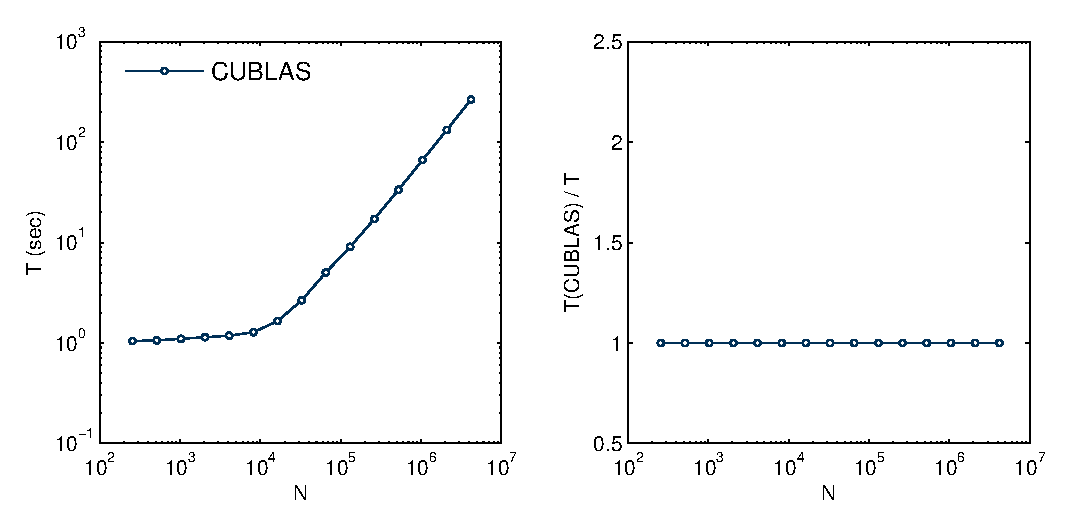
\includegraphics[width=0.9\textwidth]{perfcmp-1}}%
        \only<2> {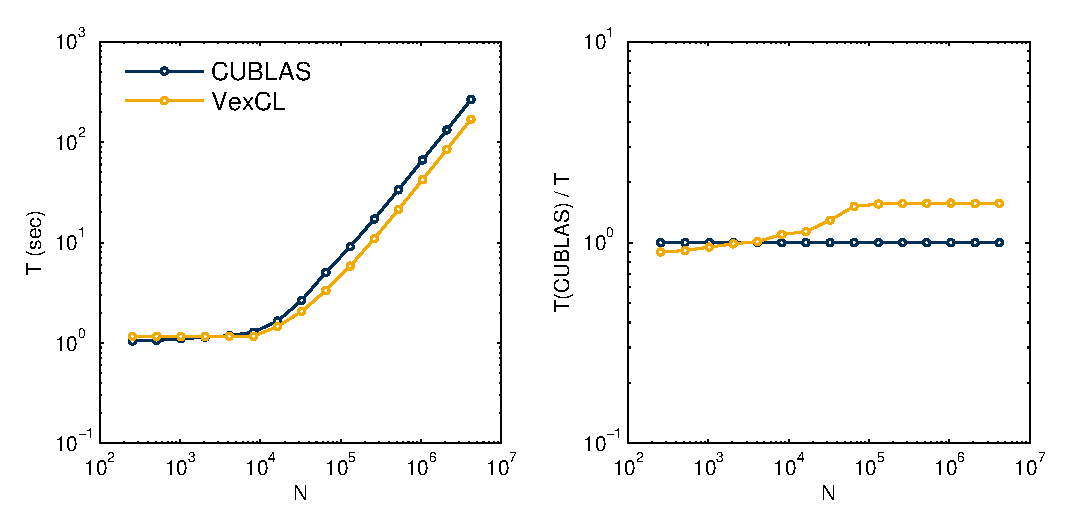
\includegraphics[width=0.9\textwidth]{perfcmp-2}}%
        \only<3> {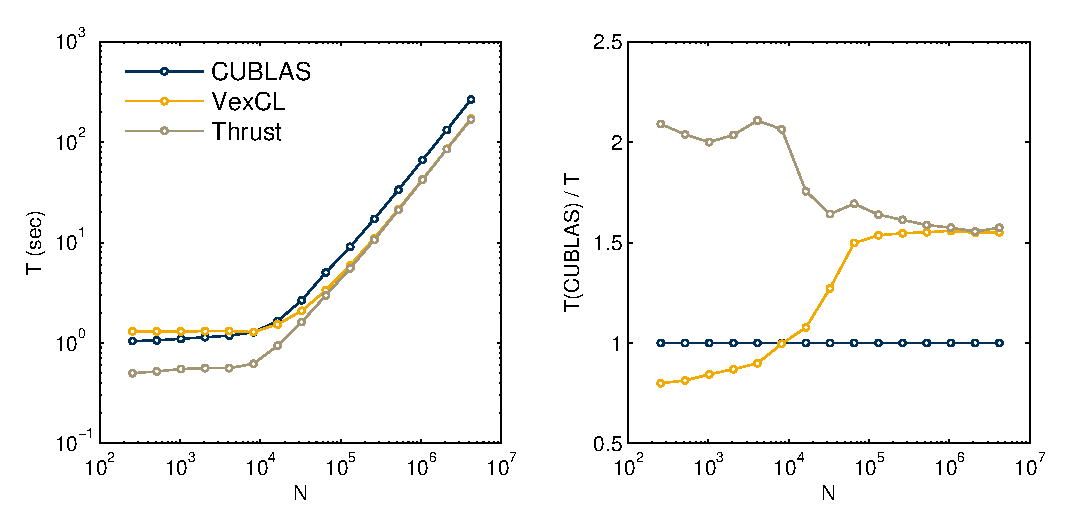
\includegraphics[width=0.9\textwidth]{perfcmp-3}}%
        \only<4->{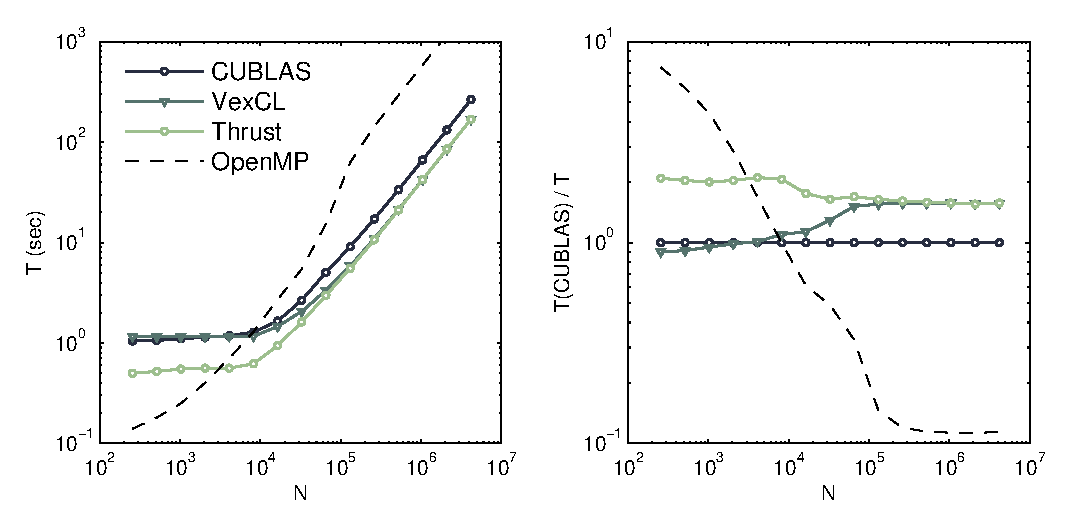
\includegraphics[width=0.9\textwidth]{perfcmp-4}}%
    \end{figure}
    \begin{uncoverenv}<5>
        \begin{itemize}
            \item Недостатки простейшей реализации:
                \begin{itemize}
                    \item Метод Рунге-Кутты использует 4 временных переменных
                        состояния.
                    \item Одна итерация метода приводит к запуску нескольких
                        ядер OpenCL.
                \end{itemize}
            \end{itemize}
    \end{uncoverenv}
\end{frame}

\note{ }

%----------------------------------------------------------------------------
\begin{frame}[fragile]{Специально написанное ядро}
    \begin{columns}
        \begin{column}{0.45\textwidth}
            \begin{itemize}
                \item Создадим монолитное ядро, соответствующее одной итерации
                    метода Рунге-Кутты.
                \item Будем вызывать ядро в цикле интегрирования.
                    \vspace{\baselineskip}
                \item Получим 10-кратное ускорение!
                    \begin{itemize}
                        \item<2|alert@2> \emph{Потеряв универсальность odeint}.
                    \end{itemize}
            \end{itemize}
        \end{column} \quad \quad
        \begin{column}{0.5\textwidth}
            \begin{exampleblock}{}
                \begin{adjustbox}{width=0.95\textwidth,height=0.95\textheight,keepaspectratio}
                    \begin{lstlisting}
double3 lorenz_system(double r, double sigma, double b, double3 s) {
    return (double3)( sigma * (s.y - s.x),
                       r * s.x - s.y - s.x * s.z,
                       s.x * s.y - b * s.z);
}
kernel void lorenz_ensemble(
    ulong  n, double dt, double sigma, double b,
    const global double *R,
    global double *X,
    global double *Y,
    global double *Z
    )
{
    for(size_t i = get_global_id(0); i < n; i += get_global_size(0)) {
        double  r = R[i];
        double3 s = (double3)(X[i], Y[i], Z[i]);
        double3 k1, k2, k3, k4;

        k1 = dt * lorenz_system(r, sigma, b, s);
        k2 = dt * lorenz_system(r, sigma, b, s + 0.5 * k1);
        k3 = dt * lorenz_system(r, sigma, b, s + 0.5 * k2);
        k4 = dt * lorenz_system(r, sigma, b, s + k3);

        s += (k1 + 2 * k2 + 2 * k3 + k4) / 6;

        X[i] = s.x; Y[i] = s.y; Z[i] = s.z;
    }
}
                    \end{lstlisting}
                \end{adjustbox}
            \end{exampleblock}
        \end{column}
    \end{columns}
\end{frame}

\note[itemize]{
\item So, what if we did this manually?
\item We would create a single kernel that would do complete Runge-Kutta
    integration step. By the way, here is the kernel that does just that. It's
    very nice-looking kernel in fact.
\item If we run this kernel in a loop, it would give us our solution. And it
    would be ten times faster than our previous variant. So a hundred times
    faster than a CPU! That's an acceleration!
\item But, odeint has 20 different steppers. We don't want to reimplement all
    of those. Let Karsten here do the job, right?
}

\section{Генератор ядер}

%----------------------------------------------------------------------------
\begin{frame}[fragile]{Генерация OpenCL-кода из алгоритмов Boost.odeint}
    \begin{itemize}
        \item VexCL включает тип \code{vex::symbolic<T>}.
        \item Любые арифметические операции с переменными этого типа выводятся
            в выходной поток:
    \end{itemize}
    \begin{exampleblock}{}
        \begin{lstlisting}
vex::symbolic<double> x = 6, y = 7;
x = sin(x * y);
        \end{lstlisting}
    \end{exampleblock}
    \begin{small}
        \begin{verbatim}
double var1 = 6;
double var2 = 7;
var1 = sin( ( var1 * var2 ) );
        \end{verbatim}
    \end{small}
    \pause
    \vspace{-1\baselineskip}
    \begin{itemize}
        \item Простая идея:
            \begin{itemize}
                \item Запишем последовательность действий алгоритма.
                \item Сгенерируем ядро OpenCL.
            \end{itemize}
    \end{itemize}
\end{frame}

\note[itemize]{
\item VexCL allows to achieve same effect without manual coding.
\item The idea is very simple:
    \begin{itemize}
        \item An algorithm (any algorithm) is just a sequence of arithmetic
            expressions.
        \item VexCL symbolic types allow to record such expressions.
    \end{itemize}
}

%----------------------------------------------------------------------------
\begin{frame}[fragile]{Запишем последовательность действий алгоритма Boost.odeint}
    \begin{exampleblock}{1. Тип переменной состояния}
        \begin{lstlisting}
typedef vex::symbolic< double > sym_vector;
typedef std::array<sym_vector, 3> sym_state;
        \end{lstlisting}
    \end{exampleblock}

    \begin{exampleblock}{2. Системная функция}
        \begin{lstlisting}[firstnumber=last]
struct lorenz_system {
    const sym_vector &R;
    lorenz_system(const sym_vector &R) : R(R) {}

    void operator()(const sym_state &x, sym_state &dxdt, double t) const {
        dxdt[0] = sigma * (x[1] - x[0]);
        dxdt[1] = R * x[0] - x[1] - x[0] * x[2];
        dxdt[2] = x[0] * x[1] - b * x[2];
    }
};
        \end{lstlisting}
    \end{exampleblock}
\end{frame}

\note[itemize]{
\item Let's record the sequence of expressions that, for example, Runge-Kutta
    method does, and let's build an OpenCL kernel from this sequence.
\item We replace the state type with array of three symbolic variables. We also
    slightly modify our system functor.
}

%----------------------------------------------------------------------------
\begin{frame}[fragile]{Запишем последовательность действий алгоритма Boost.odeint}
    \begin{exampleblock}{3. Алгоритм (Рунге-Кутты 4го порядка)}
        \begin{lstlisting}[firstnumber=last]
odeint::runge_kutta4<
        sym_state /*state*/,      double /*value*/,
        sym_state /*derivative*/, double /*time*/,
        odeint::range_algebra, odeint::default_operations
        > stepper;
        \end{lstlisting}
    \end{exampleblock}

    \begin{exampleblock}{4. Запишем одну итерацию метода Рунге-Кутты}
        \begin{lstlisting}[firstnumber=last]
std::ostringstream lorenz_body;
vex::generator::set_recorder(lorenz_body);

sym_state sym_S = {{ sym_vector(sym_vector::VectorParameter),
                      sym_vector(sym_vector::VectorParameter),
                      sym_vector(sym_vector::VectorParameter) }};
sym_vector sym_R(sym_vector::VectorParameter, sym_vector::Const);

lorenz_system sys(sym_R);
stepper.do_step(std::ref(sys), sym_S, 0, dt);
        \end{lstlisting}
    \end{exampleblock}
\end{frame}

\note[itemize]{
\item We also alter the stepper type accordingly.
\item Next we create the string stream and register it as the expression
    recorder.
\item Finally, we create symbolic variables that would correspond to generated
    kernel parameters, and run single integration step.
\item Now lorenz\_body holds the recorded expression sequence that we
    need.
}

%----------------------------------------------------------------------------
\begin{frame}[fragile]{Генерация вычислительного ядра OpenCL}
    \begin{exampleblock}{5. Сгенерируем и вызовем ядро OpenCL}
        \begin{lstlisting}[firstnumber=last]
auto lorenz_kernel = vex::generator::build_kernel(ctx, "lorenz", lorenz_body.str(),
        sym_S[0], sym_S[1], sym_S[2], sym_R);

vex::vector<double> X(ctx, n), Y(ctx, n), Z(ctx, n), R(ctx, n);

X = Y = Z = 10;
R = Rmin + (Rmax - Rmin) * vex::element_index() / (n - 1);

for(double t = 0; t < t_max; t += dt) lorenz_kernel(X, Y, Z, R);
        \end{lstlisting}
    \end{exampleblock}
\end{frame}

\note[itemize]{
\item We generate the OpenCL kernel named "lorenz" with the information from
    \code{lorenz_body}. We also supply the symbolic vectors that participated
    in our algorithm. Those will become kernel parameters.
\item Next we create our device vectors, and run the integration loop with the
    generated kernel.
\item And this could be done for any of 20 odeint steppers or for almost any
    other generic algorithm!
}

%----------------------------------------------------------------------------
\begin{frame}{Ограничения}
    \begin{itemize}
        \item Поддерживаются только строго параллельные (embarrassingly
            parallel) алгоритмы.
        \item Допускается только линейная последовательность действий
            (отсутствие ветвлений или циклов с переменным числом итераций).
        \item Возможна небольшая потеря точности при преобразовании констант в
            строки.
    \end{itemize}
\end{frame}

\note[itemize]{
\item Of course, there are some restrictions.
}

%----------------------------------------------------------------------------
\begin{frame}[fragile]{Производительность сгенерированного ядра}
    \begin{figure}
        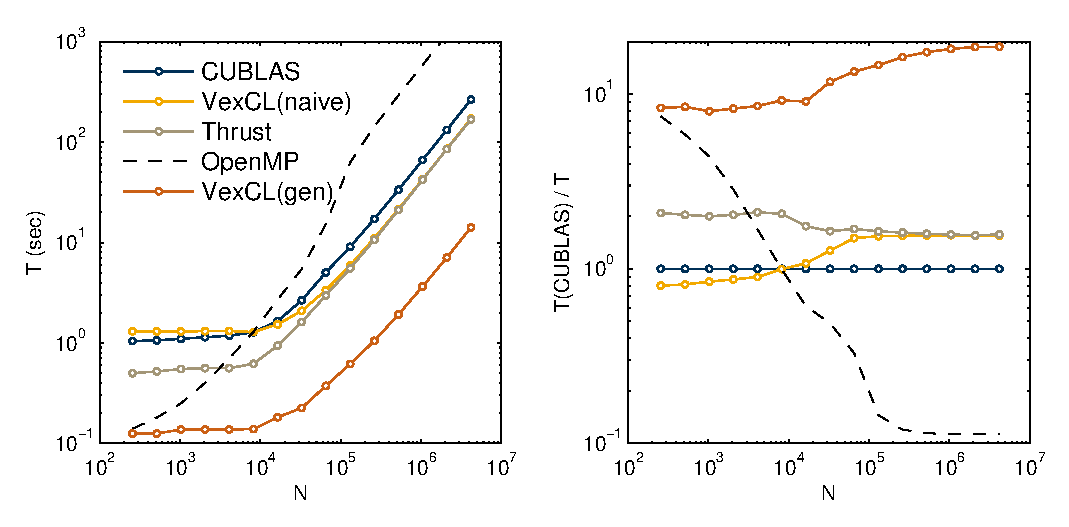
\includegraphics[width=\textwidth]{perfcmp-5}
    \end{figure}
\end{frame}

\note[itemize]{
\item But, as you can see from this slide, the technique allows to achive same
    acceleration we got from manually coded kernel (Both for CPU and GPU).
}

\section{Заключение}

%----------------------------------------------------------------------------
\begin{frame}{Некоторые проекты, использующие VexCL}
    \begin{description}[\quad]
        \item[AMGCL] --- алгебраический многосеточный метод решения СЛАУ
            \begin{itemize}
                \item \href{https://github.com/ddemidov/amgcl}{https://github.com/ddemidov/amgcl}
            \end{itemize}
            \vspace{\baselineskip}
        \item[Antioch] --- высокотемпературные термохимические расчеты
            \begin{itemize}
                \item \href{https://github.com/libantioch/antioch}{https://github.com/libantioch/antioch}
            \end{itemize}
            \vspace{\baselineskip}
        \item[Boost.odeint] --- набор обобщенных алгоритмов решения ОДУ
            \begin{itemize}
                \item \href{http://odeint.com}{http://odeint.com}
            \end{itemize}
    \end{description}
\end{frame}

%----------------------------------------------------------------------------
\begin{frame}{Заключение}
    \ghribbon
    \begin{itemize}
        \item VexCL позволяет писать прозрачный и компактный код без потери
            производительности.
        \item Генератор кода преобразует обобщенные алгоритмы \Cpp в код
            OpenCL:
            \begin{itemize}
                \item Уменьшается число обращений к глобальной памяти.
                \item Снижается число запусков вычислительных ядер.
                \item Код может использоваться как для CPU, так и для GPU
                    вариантов программы.
            \end{itemize}
            \vspace{\baselineskip}
            \vspace{\baselineskip}
        \item \href{https://github.com/ddemidov/vexcl}
            {https://github.com/ddemidov/vexcl}
    \end{itemize}
\end{frame}

\note{ }

\end{document}

% vim: et
